% 유형 02 0050(본책 13쪽) — 삼각형 ABC, AB=12 · AC=10. 스캔 삽화를 TikZ 로 다시 그림.
% 라벨은 원문 그대로(12 · 10 · 꼭짓점). 높이·BC 의 길이(답의 근거)는 적지 않는다.
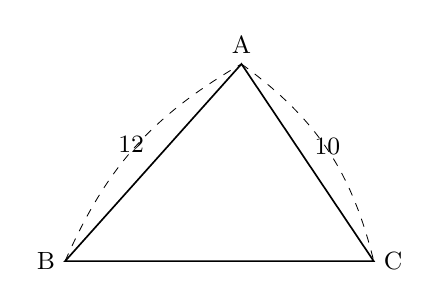
\begin{tikzpicture}[scale=0.28, line width=0.6pt]
  \coordinate (B) at (0,0); \coordinate (C) at (14,0); \coordinate (A) at (8,8.944);
  \draw (A) -- (B) -- (C) -- cycle;
  \draw[dashed, line width=0.3pt] (B) to[bend left=18] (A);
  \draw[dashed, line width=0.3pt] (A) to[bend left=20] (C);
  \node[font=\small, above] at (A) {A};
  \node[font=\small, left] at (B) {B};
  \node[font=\small, right] at (C) {C};
  \node[font=\small] at (3.0,5.3) {$12$};
  \node[font=\small] at (11.9,5.2) {$10$};
\end{tikzpicture}
